The code is written in the Arduino IDE for the Raspberry Pi Pico2.  
The project structure is as follows:

\dirtree{%
.1 treadmill\_sideshift.ino \DTcomment{Main project file}.
.1 src/.
.1 include/ \DTcomment{Classes used by main hardware handling, algorithms}.
.2 I2CCommunication.h \DTcomment{Provide I2C communication}.
.2 ICommunication.h \DTcomment{Defines communication interface}.
.2 Motor.h \DTcomment{Provide communication with the motor driver}.
.2 MotorFeedback.h \DTcomment{Reading analog feedback from motor}.
.2 OtherDevice.h \DTcomment{Defines communication message, store the last message}.
.2 Pid.h \DTcomment{PID controller with integral windup protection}.
.2 PositionCalculator.h \DTcomment{converts raw ADC readings from a motor piston sensor into a physical position}.
.2 UARTCommunication.h \DTcomment{Provide I2C communication}.
.2 UserInterface.h \DTcomment{handles buttons, potentiometer, and LED indicators}.
.1 test/ \DTcomment{Codes for solo hardware testing, other device simulation}.
.2 ICommunication\_test/.
.2 Motor\_test/.
.2 MotorFeedback\_test/.
.2 SynMode\_test/.
.2 UserInterface\_test/.
}
The properties of the classes are defined in the headers of the individual files.

\subsection{State machine}
\begin{figure}[h!]
    \centering
    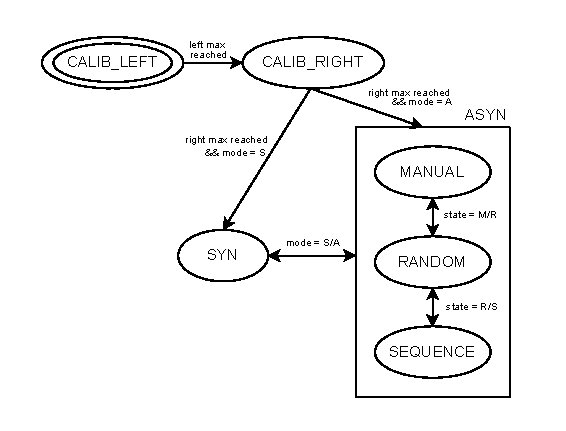
\includegraphics[width=\textwidth]{images/sideshift_state-machine.drawio.pdf}
    \caption{Sideshift state machine.}
    \label{fig:state_machine}
\end{figure}

State description:
\begin{itemize}
    \item \textbf{CALIB\_LEFT} – Initial state, used to find the maximum ADC value of the transducer, which is then stored to determine the exact position of the piston at its extreme end. The maximum is determined by running the motor until its position no longer changes for a certain period of time.
    \item \textbf{CALIB\_RIGHT} – The same, but in this case it concerns the minimum ADC value of the transducer.
    \item \textbf{SYN} – State in which the piston follows the second piston (position is known via communication). A PI controller is used to maintain zero control deviation.
    \item \textbf{MANUAL} – Manual control is active, allowing the piston to be positioned using the L/R buttons. The maximum speed is selected via a potentiometer.
    \item \textbf{RANDOM} – In random mode, a position is selected within the range of the piston rod, and a PI controller drives the rod to the selected position. After reaching the position, the next position is selected randomly. Maximum speed is set via a potentiometer.
    \item \textbf{SEQUENCE} – The piston rod moves left and right, with the maximum speed set via a potentiometer.
\end{itemize}

Transitions between states
\begin{itemize}
    \item \textbf{MAX REACHED} – The maximum (minimum) is considered reached if the motor is driven in one direction, 
    and the ADC converter value does not change by more than the interval defined in the 
    constant \texttt{changeTolerance} during the time interval defined in the constant 
    \texttt{stableThreshold}.
    \item \textbf{STATE and MODE} – These transitions depend on the position of the switches on the control panel.
\end{itemize}

\subsection{Communication}
\subsubsection{Choosing protocol}
For communication, it is necessary to correctly select the protocol, which is chosen in the \texttt{setup} loop.  
One of the following lines must be uncommented:
\begin{verbatim}
comm = new UARTCommunication();
//comm = new I2CCommunication(isMaster);
\end{verbatim}

By enabling the UART protocol, a class is created that handles the communication.  
The protocols must be the same on both boards.

\subsubsection{Message type}
Messages are sent as strings. The \texttt{OtherDevice} class handles this conversion,  
and follows these rules:

\begin{itemize}
    \item The message always starts with the character \texttt{<}.
    \item Values are separated by commas.
    \item The first value is the piston position (\texttt{pos}), represented as a floating-point number with two decimal places.
    \item The second value is the potentiometer reading (\texttt{pot}), represented as an integer.
    \item The third value is the direction (\texttt{dir}), represented as an integer.
    \item The message always ends with the character \texttt{;}.
\end{itemize}

\noindent
An example of a generated message:
\begin{verbatim}
<12.45,75,1;
\end{verbatim}

\noindent
Meaning of the message:
\begin{itemize}
    \item \texttt{pos = 12.45} $\rightarrow$ piston position in millimeters.
    \item \texttt{pot = 75} $\rightarrow$ potentiometer value in percent (75\,\% of maximum speed).
    \item \texttt{dir = 1} $\rightarrow$ piston movement direction.
\end{itemize}

\subsubsection{Communication period}
The communication period can be set by the constant \textit{COMM\_MS} in the main file. By default, it is set and tested to 50 ms.

